\chapter{Tableur}\label{ficheTableur1}  

Un tableur est un logiciel qui permet de faire des calculs à partir de tableaux contenant des nombres (les \emph{données}). Un tableur permet également de représenter ces données sous forme de graphiques qui en facilitent généralement la lecture.\\

\prof{On pourra ici indiquer qu'il existe plusieurs logiciels de tableur, celui que nous allons utiliser étant le plus connu : Excel, contenu dans le pack Office de Microsoft. Un autre tableur très utilisé est Calc, de la suite LibreOffice. Il présente l'avantage d'être libre et gratuit. L'utilisation de nombreuses fonctions est la même pour ces deux logiciels.}

{\footnotesize
\begin{itemize}
\item Logiciel : \emph{Microsoft Excel}
\item Prérequis : aucun
\item Matières concernées : mathématiques, physique-chimie, histoire-géographie
\item Objectifs : utiliser un tableur pour traiter des données, les visualiser sous forme de graphique et préparer un compte rendu au format PDF remis sur Teams.
\item Compétences : 
        \begin{itemize}
        \item insérer une formule ;
        \item utiliser la recopie incrémentale ;
        \item tracer un graphique ;
        \item exporter au format PDF.
        \end{itemize}
\item Cette fiche est à réaliser :
        \begin{itemize}
        \item avant les vacances d'octobre en mathématiques ;
        \item avant les vacances de Noël en physique-chimie ;
        \item avant la fin du semestre de cours en histoire-géographie. 
        \end{itemize}
\prof{\item vous devez préparer un élément \underline{avant} la séance : un devoir sur Teams où vos élèves déposeront le résultat de leur activité sous la forme d'un fichier PDF.}
\end{itemize}
}


\newpage


\section{Séance 1 : évolution des notes d'un élève}


\subsection{Premiers pas avec Excel}\index{Ouvrir!Calc}

Lancer le logiciel en utilisant la <<\,loupe\,>> (voir ci-dessous) ou en appuyant simultanément sur cmd et espace :

\uneimageici{./images/generales/loupe}{.7\textwidth}

... puis en indiquant \emph{Excel} :

\uneimageici{./images/tableur/loupe_recherche_Excel1}{.7\textwidth}

Choisir \emph{Microsoft Excel.app} dans la liste proposée :

\uneimageici{./images/tableur/loupe_recherche_Excel2}{.5\textwidth}

On arrive alors dans la fenêtre principale du tableur qui contient une \emph{feuille de calcul} vide :

\uneimageici{./images/tableur/CalcPresentation_Excel_crop}{.9\textwidth}

\prof{Faites manipuler les cellules aux élèves, leur faire par exemple remplir la cellule \texttt{AA30} avec un nombre de leur choix, pour qu'ils doivent utiliser les ascenceurs. Montrez aux élèves comment redimensionner une colonne ou une ligne, plusieurs colonnes ou plusieurs lignes (en les sélectionnant auparavant), toutes les colonnes ou toutes les lignes (en les sélectionnant toutes).}


%
%
%  S  É  A  N  C  E     I
%
%


\subsection{Pour bien démarrer...}

Dès que vous avez ouvert un nouveau document dans \emph{Excel}, sauvegardez-le au format Nom-date.xlsx : dans le menu \texttt{Fichier}, choisir \texttt{Enregistrer}. Pendant que vous travaillez, pensez à sauvegarder régulièrement votre travail (raccourci clavier \texttt{Cmd + s}).   

\uneimageici{./images/generales/clavierCmdS}{.4\textwidth}


\subsection{L'activité demandée}

\prof{Assurez-vous que tous les élèves aient franchi les premières étapes ci-dessus. Lire ensuite l'énoncé avec les élèves et montrer le résultat attendu (affichage au TBI du résultat). À partir de ce point, les élèves travaillent chacun à son rythme.}

\boiteEnonce{Au cours d'une année scolaire, un élève a obtenu les notes suivantes sur 20 points : \[11\quad 15\quad 12\quad 18\quad 16\quad 13\quad 8\quad 15\] On souhaite réaliser un graphique qui montre l'évolution de ses notes au cours de l'année et calculer ensuite sa moyenne annuelle. L'objectif est d'obtenir le résultat suivant :
\uneimageici{./images/tableur/CalcSituationFinaleMaths_Excel_crop}{.75\textwidth}
Une fois votre travail terminé, vous devrez exporter votre fichier au format PDF (le fichier doit être nommé à partir de votre nom : \texttt{Nom-date.pdf}) puis vous le rendrez sur Teams à l'endroit indiqué par votre enseignant (si nécessaire, se reporter à la fiche méthode \emph{Remettre son devoir}, page \pageref{TeamsRemettreDevoir}).}

\textbf{Pour obtenir de l'aide, rendez-vous à la page \pageref{aideExcel}}

\subsection{Pour aller plus loin...}

Après avoir terminé, faire des tests :

\begin{itemize}
\item modifier les notes et observer les modifications de la courbe ;
\item exporter le graphique en tant qu'image (sélectionner le graphique, cliquer sur le graphique avec le bouton droit, puis choisir \texttt{Enregistrer en tant qu'image...}) ;\index{Calc!Exporter un graphique comme image}\index{Exporter un graphique comme image (Calc)}
\item mettre en forme la feuille de calcul pour qu'elle ressemble à l'image présentée ci-dessous.
\end{itemize}


\uneimageici{./images/tableur/CalcPourAllerPlusLoin_Excel_crop}{.7\textwidth}


\newpage

\section{Aide pour réaliser les activités}\label{aideExcel}

\subsection{Aide pour la séance 1}

\subsubsection{Entrer les données}

\begin{itemize}
\item Cliquer dans la cellule \texttt{A1}.
\item Taper au clavier le texte qui doit être contenu dans la cellule : \texttt{numéro du test}.
\item Cliquer dans la cellule \texttt{B1} et écrire le premier numéro du test : 1.
\item Cliquer dans la cellule \texttt{C1} et écrire le deuxième numéro du test : 2.
\item Utiliser la \emph{recopie incrémentale}\index{Recopie incrémentale (Calc)}\index{Calc!Recopie incrémentale} pour remplir les cellules suivantes : pour cela, sélectionner les deux cellules (B1 et C1). Approcher le curseur de la souris du coin inférieur droit de la cellule \texttt{C1}. Lorsque le curseur se change en croix
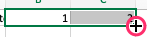
\includegraphics[scale=.4]{./images/tableur/recopieIncrementale_Excel_crop}, cliquer et tirer (en maintenant cliqué) vers la droite pour remplir les cellules suivantes jusqu'à la valeur 8 (voir image ci-dessous).
\end{itemize}

\uneimageici{./images/tableur/recopieIncrementale_Excel2_crop}{\textwidth}

\begin{itemize}
\item Cliquer dans la cellule \texttt{A2} et écrire \texttt{note sur 20}.
\item Remplir les cellules de la ligne 2 avec les notes correspondant aux différents tests.
\end{itemize}





\subsubsection{Sauvegarder le fichier}
\label{ssec_sauvegarder_fichier}
Il est important de sauvegarder régulièrement le fichier sur lequel on travaille.


Pour enregistrer votre travail :
\begin{itemize}
\item Ouvrir le menu \texttt{Fichier}.
\item Choisir \texttt{Enregistrer sous...}
\item Entrer le nom du fichier sous la forme \texttt{Nom-date}. \circled{1}
\item Cliquer sur \texttt{Sur mon Mac} pour choisir où enregistrer le fichier. Cela transforme la fenêtre. \circled{2}
\item Choisir comme emplacement le \emph{Bureau} de l'ordinateur. \circled{3}
\item Vérifier que le fichier est bien enregistré au format \emph{Classeur Excel (.xlsx)}. \circled{4}
\end{itemize}

\uneimageici{./images/tableur/CalcEnregistrerFichier_Excel1_crop}{.7\textwidth}

\uneimageici{./images/tableur/CalcEnregistrerFichier_Excel2_crop}{.9\textwidth}

Une fois cela fait, appuyer régulièrement sur la combinaison de touche \texttt{cmd} + \texttt{S} : c'est le \emph{raccourci clavier} permettant d'enregistrer votre travail.

\uneimageici{./images/generales/clavierCmdS}{.5\textwidth}



\cadre{\textbf{Différence entre \texttt{Enregistrer} et \texttt{Enregistrer sous...}}\newline Dans la plupart des logiciels, on peut : \begin{itemize}\item \textbf{Enregistrer} le fichier sur lequel on travaille. Cette opération est possible si le fichier existe déjà et possède un nom. La version courante du fichier sera alors sauvegardée et remplacera l'ancienne version du fichier.
\item \textbf{Enregistrer sous...} le fichier sur lequel on travaille. Cette opération commence par demander un nouveau nom pour l'enregistrement du fichier. On peut donc ouvrir un fichier que l'on ne souhaite pas modifier, choisir \emph{enregistrer sous}, donner un nouveau nom et ainsi travailler sur une copie du fichier de départ.
\item utiliser \texttt{cmd + s} (\emph{s} pour \emph{Save}) pour \textbf{enregistrer} le fichier courant. Bien que les documents soient enregistrés automatiquement par la majorité des logiciels, il faut régulièrement sauver son travail pour éviter les surprises.\end{itemize}}









\subsubsection{Créer un graphique}\index{Calc!Créer un graphique}\index{Créer un graphique (Calc)}

\begin{itemize}
\item Sélectionner les données à représenter : cliquer sur la cellule \texttt{B1} et tirer (en maintenant cliqué) jusqu'à la cellule \texttt{I2}. Les cellules sélectionnées apparaissent en gris.
\uneimageici{./images/tableur/CalcCellulesSelectionnees_Excel_crop}{.9\textwidth}

\item Cliquer alors sur l'onglet \texttt{Insertion}\circled{1} puis sur l'icône représentant le type de graphique souhaité. Dans notre cas, ce sera un graphique de courbe 2D. \circled{2} Plusieurs types de graphiques s'affiche. Choisir le graphique \texttt{Courbe avec marques}. \circled{3}
\uneimageici{./images/tableur/CalcBoiteDiagramme1_Excel_crop}{.6\textwidth}
\end{itemize}

Vous avez maintenant un graphique qui s'est ajouté dans la feuille de calcul. Attention, la fenêtre du graphique est sélectionnée, ce qui est visible grâce aux huit poignées de sélection qui entourent la fenêtre :

\uneimageici{./images/tableur/CalcFenetreGraphiqueSelectionnee_Excel_crop}{.6\textwidth}

Pour déplacer la fenêtre graphique, déplacer la souris sur le bord pour qu'apparaisse sur le curseur une croix. Le déplacement s'effectue en maintenant cliqué et en déplaçant la souris. Pour revenir à la feuille de calcul, cliquer sur n'importe quelle cellule (les poignées de sélection disparaissent alors).

Nous devons à présent corriger les valeurs du graphique, car elles ne correspondent pas à ce que nous avons envie. En effet, il ne faudrait avoir qu'une courbe, dont les points représentent la relation entre nos deux lignes. Pour commencer, il faut supprimer la droite qui est en bleu sur ce graphique. Il suffit pour cela de cliquer dessus. Ses sommets seront alors mis en évidence (comme sur l'image ci-dessous). Une fois cela fait, appuyez sur la touche \texttt{retour} (au-dessus de la touche \texttt{entrée}).

\uneimageici{./images/tableur/Calc_supprimer_courbe_Excel_crop}{.6\textwidth}

À présent, pour corriger les valeurs de la courbe que nous avons déjà, il faut la sélectionner en cliquant dessus. Là aussi, ses points seront mis en évidence. Il faut ensuite cliquer du bouton droit de la souris sur la courbe pour faire apparaître une liste d'options. Sélectionner \texttt{Sélectionner des données...}.

\uneimageici{./images/tableur/Calc_corriger_donnees_Excel_crop}{.6\textwidth}

Dans la fenêtre qui apparait, il faut indiquer les valeurs de l'axe horizontal du graphique. Cliquer sur le bouton à la fin du champ de texte pour sélectionner directement les valeurs sur la feuille de calcul.

\uneimageici{./images/tableur/Calc_selectionner_donnees_Excel_crop}{.6\textwidth}

Sélectionner les données des cellules \texttt{B1} à \texttt{I1} en cliquant sur la première et en déplaçant le curseur jusqu'à la dernière sans relâcher le bouton de la souris. \circled{1} Vous apercevrez la requête équivalente apparitre dans la barre de saisie de données, ce qui prouve que vous avez bien sélectionné les cellules. \circled{2}

\uneimageici{./images/tableur/Calc_selectionner_donnees_X_crop}{.6\textwidth}

De retour sur la fenêtre précédente, cliquez sur \texttt{OK} en bas, pour valider votre action.

\prof{Le graphique avait déjà les bonnes valeurs sur l'axe horizontal, mais ce ne sera pas toujours le cas.}

Pour ajouter des titres aux axes, il faut d'abord sélectionner le graphique (à nouveau, vérifiez que les poignées de sélection sont bien présentes autour de celui-ci) et cliquer sur \texttt{Ajouter un élément au graphique} dans l'onglet \texttt{Création de graphique}. \circled{1} Choisir ensuite \texttt{Titres des axes} \circled{2} puis \texttt{Horizontal principal} et \texttt{Vertical principal} pour faire apparaître les titres sur les deux axes. \circled{3}

\uneimageici{./images/tableur/Calc_ajouter_titres_axes_crop}{.6\textwidth}

Pour modifier ces titres, il suffit de cliquer dessus, sélectionner le texte et écrire le nouveau titre en remplaçant l'ancien.

\subsubsection{Calculer la moyenne}\index{Moyenne (calcul de la)}\index{Calc!Moyenne (calcul de la)}

\begin{itemize}
\item Cliquer dans la cellule \texttt{A4} et entrer le texte : \texttt{Moyenne}. \circled{1}
\item Cliquer dans la cellule \texttt{B4} dans laquelle nous allons entrer une formule : \circled{2}
        \begin{itemize}
        \item taper un signe \texttt{=} qui signifie que la cellule va contenir une formule ;
        \item Taper le nom de la formule suivie d'une parenthèse ouvrante : \texttt{=MOYENNE(} ;
        \item à l'aide de la souris, sélectionner dans la feuille de calcul les cellules contenant les notes dont on veut calculer la moyenne (voir image ci-dessous \circled{3}) ;
        \uneimageici{./images/tableur/CalcCalculMoyenne_Excel_crop}{.8\textwidth}
        \item appuyer sur la touche \texttt{Entrée} : la moyenne calculée apparaît.
        \end{itemize}
\end{itemize}



\subsubsection{Exporter au format PDF}\index{Calc!Exporter au format PDF}\index{PDF (exporter au format) (Calc)}

Une fois le travail achevé et sauvegardé, il faut exporter le fichier au format PDF. Pour cela, il faut passer par le menu \texttt{Fichier} et choisir \texttt{Enregistrer sous...} comme si vous vouliez enregistrer un nouveau fichier. La seule différence avec les étapes présentées à la page \pageref{ssec_sauvegarder_fichier}, c'est qu'il faut indiquer que le type de fichier est \texttt{PDF}. 

\uneimageici{./images/tableur/Exporter_PDF_crop}{.7\textwidth}

\cadre{Le \textbf{format PDF} est un format parfaitement adapté aux échanges de documents : il est non modifiable et lisible sur tous les périphériques (ordinateurs, tablettes, smartphones). Il peut contenir du texte, des images, des liens vers l'internet et même des vidéos ou du son. \newline À chaque fois qu'il faut rendre ou envoyer un document qui n'est pas destiné à être modifié, il faut privilégier le format de fichier PDF.}  





\subsubsection{Remettre le travail achevé sur Teams}

Une fois le travail terminé et exporté au format PDF, il faut le remettre au professeur. Pour cela, se connecter à Teams et accéder à l'équipe du cours. Cliquer sur \texttt{Devoirs} et cliquez sur le devoir correspondant à l'acvitité que vous êtes en train de terminer. Cliquez sur \texttt{Ajouter un travail}, en bas, puis \texttt{Charger à partir de cet appareil}, en bas à gauche. Sélectionnez le fichier au format PDF que vous venez d'exporter et \texttt{Ouvrir}. Une fois le travail chargé, cliquez sur \texttt{Terminé}, en bas à droite. Enfin, cliquez sur \texttt{Remettre}, en haut à droite.\\



Si nécessaire, se reporter à la fiche méthode \emph{Remettre un devoir sur Teams}, page \pageref{TeamsRemettreDevoir}.



\poubelle{

\newpage

%
%
%  S  É  A  N  C  E     II
%
%




\section{Séance 2 : Suivi en température d'une solidification}\label{ficheTableur2}

\subsection{Pour bien démarrer...}

\prof{réalisez l'expérience avec vos élèves avant la séance, ou apportez le matériel correspondant à l'expérience pour donner du sens à la séance. De même, expliquez aux élèves les résultats obtenus. Il faut bien inciter les élèves à utiliser la recopie incrémentale pour générer les temps de 0 à 10 minutes.}



\boiteEnonce{On place un tube à essai qui contient de l'eau distillée et un thermomètre dans un mélange réfrigérant. 
\uneimageici{./images/tableur/calcPhyChiSchema}{.4\textwidth}
On relève alors la température de l'eau toutes les minutes. Les résultats obtenus sont reportés dans le tableau ci-dessous.
\begin{center}
\begin{tabular}{|c|c|c|c|c|c|c|c|c|c|c|c|}
\hline
temps $t$ (min) & 0 & 1 & 2 & 3 & 4 & 5 & 6 & 7 & 8 & 9 & 10 \\ \hline
température $T$ (\degre C) & 15 & 8 & 3 & 0 & 0 & 0 & 0 & 0 & $-1$ & $-3$ & $-5$ \\
\hline
\end{tabular}
\end{center}
On souhaite réaliser un graphique qui montre l'évolution de la température (en ordonnée) en fonction du temps (en abscisse). Le résultat à obtenir est présenté ci-dessous :
\uneimageici{./images/tableur/calcPhyChi}{.7\textwidth}
Une fois votre travail terminé, vous devrez exporter votre fichier au format PDF (le fichier doit être nommé à partir de votre nom : \texttt{Nom-date.pdf}) et le rendre sur Teams.
}




\newpage



%
%
%  S  É  A  N  C  E     III
%
%




\section{Séance 3 : Évolution de la population mondiale}\label{ficheTableur3}

\subsection{Pour bien démarrer...}

\subsection{L'activité demandée}

\boiteEnonce{La population mondiale au fil du temps est reportée dans le tableau ci-dessous.
\newline
\phantom{rien}
\newline
{\footnotesize
\begin{tabular}{|p{3.5cm}|c|c|c|c|c|c|c|c|c|c|}
\hline
Dates (années) & 0 & 400 & 1000 & 1500 & 1700 & 1800 & 1850 & 1900 & 1950 & 1980  \\ \hline
Population mondiale & \multirow{2}{*}{250} & \multirow{2}{*}{200} & \multirow{2}{*}{300} & \multirow{2}{*}{480} & \multirow{2}{*}{640} & \multirow{2}{*}{900} & \multirow{2}{*}{1300} & \multirow{2}{*}{1700} & \multirow{2}{*}{2700} & \multirow{2}{*}{4400} \\
 (en millions) & & & & & & & & & & \\   
\hline
\end{tabular}
%
\newline
\phantom{rien}
\newline
%
\begin{tabular}{|p{3.5cm}|c|c|c|c|c|c|}
\hline
Dates (années) & 1990 & 2000 & 2005 & 2010 & 2015 \\ \hline
Population mondiale & \multirow{2}{*}{5300} & \multirow{2}{*}{6100} & \multirow{2}{*}{6500} & \multirow{2}{*}{6900} & \multirow{2}{*}{7400} \\
(en millions) & & & & & \\  
\hline
\end{tabular}
} % fin du footnotesize tableau
%
\newline
{\tiny\emph{Source : Wikipédia (Population mondiale) et ONU (World Population Prospects http://esa.un.org/unpd/wpp/)}}
%
\newline
\phantom{rien}
\newline
On souhaite représenter l'évolution de la population mondiale depuis le début de notre ère. On veut afficher la population en millions d'individus (en ordonnée) en fonction de l'année (en abscisse).\newline Une fois votre travail terminé, vous devrez exporter votre fichier au format PDF (le fichier doit être nommé à partir de votre nom : \texttt{Nom-date.pdf}) et le rendre sur la plateforme Moodle.
}

\prof{cette fois-ci les élèves ne voient pas le graphique à obtenir. Rappelez bien qu'il faut donner des noms aux axes (définir des étiquettes pour les axes), donner un titre au graphique. Interprétez avec les élèves le résultat obtenu. Le graphique que l'on doit obtenir est le suivant :\uneimageici{./images/tableur/calcHistoireGeoGraphique}{.7\textwidth}}
}
% il faut mettre un calcul de moyenne

% Pour aller plus loin : Europe vs Monde
